\documentclass[mestrado]{pacotes/unb-cic}
\usepackage[english,american,brazil]{babel}
\usepackage[T1]{fontenc}
\usepackage{indentfirst}
\usepackage{natbib}
\usepackage{xcolor,graphicx,url}
\usepackage[utf8]{inputenc}
\usepackage{booktabs} % for tables
\usepackage{verbatim} %% multiline comments
\usepackage{dirtytalk} %% Quotes
\usepackage{pacotes/tikz-uml} % UML
\usepackage[ruled,linesnumbered]{algorithm2e} %Algorithms
\usepackage{listings}
\usepackage{caption}
\usepackage[autostyle]{csquotes}
\usepackage{setspace}%%% more space for advisor notes

\graphicspath{ {imagens/} } % path to images

%\bibpunct[; ]{(}{)}{,}{a}{}{;}%muda colchetes para parenteses

% definicoes previas do documento
%\selectlanguage{brazil}
%\title{A Runtime model and middleware for requirements-, structure- and context-aware systems }


%\coordenador[a]{\prof[a] \dr[a] Alba Cristina Magalhaes Alves de Melo}{CIC/UnB}

\orientador[a]{\prof[a] \dr[a] Genaina Nunes Rodrigues}{CIC/UnB}
\diamesano{25}{Setembro}{2015}
\author{Gabriel Siqueira Rodrigues}
\title{A Goal-Oriented Middleware for Dependable Self-Adaptive Systems}


%\membrobanca{\prof }{CIC/UnB}

%\membrobanca{\prof }{CIC/UnB}


%\CDU{004.4}

\palavraschave{dependabilidade, deployment, sistemas autoadaptativos, sistemas autonômicos, engenharia de requisitos orientada a objetivos}
\keywords{dependability,deployment,self-adative systems, autonomic systems, goal oriented requirements engineering}

%-------------------------------------------------

\begin{document}

%\maketitle

\pretextual
%\begin{agradecimentos}
%Agradecemos à nossa orientadora, \prof[a] \dr[a] Genaina Nunes Rodrigues,
%\end{agradecimentos}

%\begin{resumo}
%Nesse trabalho apresentamos...
%\end{resumo}

% \selectlanguage{american}
%
 \begin{abstract}\textbf{}
   %- visão geral do contexto.
   We see a growing interest in computing applications that should rely on a dynamic computing environment. This computing environment can be distributed, heterogeneous and composed of not reliable computing resources.
   Theses characteristic could potentially lead to a complex deployment process. Also, in such systems, for different reasons, it could not be desirable that the system is managed by humans. We proposed in this work a method for an autonomic deployment process that allow systems to deploy itself by reflecting about its goals and its computing environment.

%
% In recent years, we see a growing availability of devices with computer capabilities. Along with this advent, comes out an opportunity to develop and deploy applications that explore those devices in dynamic environments. However, such environments are inherently characterized by uncertainty, in particular from the perspective of the system designer. To design dependable solutions for environments with a high level of uncertainty, we need models at runtime to represent the system structure, requirements as well as the system's contexts of operation in an integrated way. In addition, we need methods to reason about the system levels of operation and change them at runtime, whenever needed. In this work, we propose to address those issues by devising a component-based model approach for self-adaptation relying on GORE (goal-oriented requirements engineering) and a component-based architecture model. By these means, we plan to develop a middleware that follows and implements that model. Last, but not least, the middleware we will provide fault tolerance strategies to build a foundation for dependable systems.
%
%   To design dependable solutions to environments with a high level of uncertainty we need models to represent system structure, requirements, context in an integrated way. We need also methods for reason about the system method and change it.
%
%   %We propose a model based on Goal-Models and component-based architecture in the direction of fulfill this need. We will also develop a middleware that will keep that model. On top of that middleware we will provide fault tolerance strategies to build a foundation for dependable systems.
% %%%%%%%%%
%   % In a non-adaptive computer systems the computer is static linked to its function in the system.  To achieve a hight level of dependability in such systems one would either rely on right dependable units or on a hight level of redundancy. Both this solutions genearly leads to expensive systems. Appling self-adaptiveness is possible to a system tolerate to failures without a proibit level of redundancy. allow the development of dependable multi-processor heterogeneous systems in face of not dependable units with a lower level of redundancy.
%
%   % Our approach is a middleware that permit uses a  multi-agent runtime goal model, in witch agents can accomplish goals by selecting strategies in its local strategies repository, evaluating them by a utility function. On top of this we aim at easy the development of adaptable open-systems applications, allowing runtime discovery of peers and opportunistically sharing tasks between them, easy integration of new functional strategies and easy integration of new adaptation strategies.
%
%
\end{abstract}
%
% %\selectlanguage{brazil}
% \tableofcontents
% \listoffigures
% %listoftables
%
% \textual

\begin{document}
\capa
\sumario
%\doublespacing%%%%% Vide comentário no pacote setspace acima.
\newpage

\chapter{Introduction}
% (.5p)
\section{Introduction}
As the frontier of computing system expands to more aspects of human life we get more systems that is meant to run in dynamic computing environment. Developing software for such environment is challenging~\cite{baresi_toward_2006}.

Example of domains that leads towards dynamic environments are Ubiquitous Computing~\cite{bell_yesterdays_2007}, Internet of Things (IoT)\cite{atzori_internet_2010}, Assisted Living\cite{kleinberger_ambient_2007}, and Opportunistic Computing\cite{smaldone_improving_2011}. In such domains, the computing environment is dynamic as computer nodes can enter and leave the application. Also the computing environment can be highly heterogeneous as users have different sets of devices with different resources and characteristics. In addition, some characteristics of the computing environment can be unknown at design-time. For example, in a smart home application developer can know very little about the set of devices in the end-user home computing network.

Software deployment is the process of get a software ready to user in a given computing environment. Software deployment involves planning the deployment by assigning roles to a given computer node, selecting artifacts that must be present in the node and services that in must provide and consume. Also software deployment evolves copying artifacts for a target computing environment and setting appropriate configurations.

Traditionally software deployment is considered and human-centered activity only once executed. Such traditional view do not fit a dynamic computing environment, because in such environment the deployment should be adapted frequently. Previous works have explored goal-driven adaptation of dynamic systems at different aspects, such as configuration, behavior and structure\cite{yu_goals_2008}. Although, there is still a lack of proposals for platforms to handle autonomous deployment for dynamic environments.


%Some works model how context relate to system requirements [Rain and Dalpiaz works]. Other works use pre-designed plans to change the system architecture to respond to context changes [architecture based adapatiaion references]. Ali et al. \cite{ali_requirements-driven_2014}

%In our ongoing research, we use goal model as a solution for requirements reflection \cite{bencomo_requirements_2010}. Using this approach, we keep a requirements representation as a runtime artifact and can reflect about it during execution in order to decide on adaptations.

%We also use concepts from multiagent systems. Multiagent reasoning can lead to distributed, scalable system without a single point of failures. The advantages of using a MAS approach is the distributed nature of the system and to avoid have a sigle point of failure.

 %In special, we are interested in self-assembly and fault-tolerance in decentralized systems. This work focus on a conceptual model for implement systems with self-assembly and fault-tolerance.

%To make opportunistic computing a reality, middleware services must mask disconnections and delays and manage heterogeneous computing resources, services, and data to provide a uniform view of the system to the applications.\cite{conti_opportunities_2010}


% TODO Advantages of our approach

%In this paper, we will focus on deployment planing, for handling variability in the computing environment.
%We extend goal models with concept of resource dependency and system components. We propose a method for plan a deployment given a set of system goals, system components and available resources.


\section{Problem}
In a dynamic computing environments the system is required to constantly deploy and adapt, as goals and resources change. This is opposite to the traditional view  in with is expected that deployment is a human centered task executed only once.
This work focus on the following challenges related to deployment in dynamic computing environments:

\label{sec:problem}
%\section{Challenges}
\label{sec:challenges}

\textbf{ Challenge 1: heterogeneous computing environment.}: the system is mean to run in a broad range of configurations of the computing environment.

\textbf{ Challenge 2: uncertainty at design time.} The system developer do not know the exact specification of the end user computing environment. This call for using abstract models of environment variability.

\textbf{ Challenge 3: dynamism.} Nodes and resources can enter and leave the environment. In response, the system should constant adapt to keep hight level goals achievable despite changes in the environment.

\textbf{ Challenge 4: openness.} Third party developers should be able to develop components to the system. The objective here is achieve decentralization and independence of provider. According, the system should not drive adaptation relying on models that can not be extensible at runtime.

\textbf{ Challenge 5: deployment specification accessible to users.} Users may change their goals in a given environment and lead to the need to deployment change. A system administrator with knowledge in software deployment could be not available.



\section{Proposed Solution}
This work propose a method for autonomous deployment driven by context-goal model. Software centered systems that adopt this approach are able to accept goals, evaluate its capabilities and context and find the software modules that enable it to achieve its goals, fetch and install them. Also, the system can at runtime change its deployment in response to changes in its context, capabilities and available software modules.

%TODO: Why deployment matters
% executed multiple times during development and test.

The presented approach leverage context-goal models as the model that driven the adaptation. Goal modeling is an approach for system requirements that model the intentionality of actors.
%Goal-driven introspectiveness are a promising approach in dynamic systems. Goal-driven introspective system can reason about its goals at runtime and adapt to tackle changes in the environment.
Context runtime goal models insert the context as another dimension, modeling the variability of interest in the environment as context an how it affect the system goals and means of achieving its goals.
%The advantages of goal-driven adaptation is the high level of flexbility and easy the development by reuse the goal model.
Using Context-goal models to driven the deployment, we can avoid rework by reusing a model already developed in a requirements eliciting stage. Also, because goal-models are highly abstract models, we can achieve a higher level of flexibility. In addition, by using user goals as a drive of adaptation we expect to make deployment configuration accessible to users, even if they do not have technical skills in system administration.

%The idea is that with a support of a self-adaptive framework the system can achieve a high degree of autonomy in its deployment, allowing not specialized users configure the deployment by choosing the goals that they want to achieve in a given computing environment.
To execute the adaptation we propose the use of component-based adaptation in which the system is adapted by binding and unbinding software components at runtime. We find it promising as a component present a good level of abstraction (opposed to code or variable levels). It also builds upon mature component-based software engineering.

To allow open and decentralized evolution of the system we avoid the use of centralized design time models. Instead we propose break strategies to achieve goals as components that can be discovered at runtime. So third party developers can provide new components for achieve goals using different set of resources.

In order to easy the development of solutions that use the approach proposed in this work we are developing a reusable framework. The framework should have much the adaptation logic needed for the autonomous deployment.


%\section{Problem Definition}

% is there any component model suitable to trace goals and component service.

To allow the system make decisions about its structure based on requirements and context we need a model that can correlate this 3 concepts: the system structure, the requirements and the context.

What leads us to or general question:


\setlength{\fboxsep}{10pt}
\noindent\fbox{%
    \parbox{0.95\textwidth}{%
        \textbf{Research Question 1 (RQ1):} What would be a good model of software system that
        could allow for reason about the system structure, context and trace the requirements at runtime? In another words, represent the system requirements, structure, operation context and the relationship between this elements?
    }%
}\bigskip

As this question is too difficult to answer directly we will make a proposal of solution and evaluate it. In this work we choose to represent requirements in a Goal Model based approach, the system structure from an architectural point of view and the context as a data reference resolution process.


\setlength{\fboxsep}{10pt}
\noindent\fbox{%
    \parbox{0.95\textwidth}{%
        \textbf{Research Question 2 (RQ2):} Would a model that represent system requirements at runtime as goals, system organization at a component level and a context as a data reference resolution process a model that satisfy RQ1?
    }%
}\bigskip

Yet in relation to RQ1, to develop what would be a good model we did more questions in relation to the fitness of the model for the purpose of decide on system adaptations. The following is in direction of find if a given configuration of the system is valid.

\setlength{\fboxsep}{10pt}
\noindent\fbox{%
    \parbox{0.95\textwidth}{%
        \textbf{Research Question 3 (RQ3):} How to, using the model from RQ1, verify if systems goals are achievable at runtime in face of deployment (configuration) uncertainty.
    }%
}\bigskip

Beside check the system validity in other to forecast faults we want to be able to tolerate faults. What leads to the next question:

\setlength{\fboxsep}{10pt}
\noindent\fbox{%
    \parbox{0.95\textwidth}{%
        \textbf{Research Question 4 (RQ4):} How to assure that goals are always achieved, if they are achievable, in face of components faults ?
    }%
}\bigskip

This research question is the search to insert fault-tolerance, to achieve dependability of the system in face of not dependable components. To achieve a greater level of manutenability, the faul-tolerance techniques should be portable.


\setlength{\fboxsep}{10pt}
\noindent\fbox{%
    \parbox{0.95\textwidth}{%
        \textbf{Research Question 5 (RQ5):}	Is it feasible to implement fault tolerance techniques (\textit{retry, retry on alternate resource, check-
point/restart and replication}) as portable components that plug in the runtime model of the system?
    }%
}\bigskip

We also want to asses if the model is a practical solution.

\setlength{\fboxsep}{10pt}
\noindent\fbox{%
    \parbox{0.95\textwidth}{%
        \textbf{Research Question 6 (RQ6):} The model could be used to build a middleware that allows systems build on top of it to asses itself capacity of fulfill their requirements, self-heal in case of not and tolerate faults?
    }%
}\bigskip

As a side goal, we want to build a community around the middleware tool so we can evaluate it practical value for development of systems by third party.

\setlength{\fboxsep}{10pt}
\noindent\fbox{%
    \parbox{0.95\textwidth}{%
        \textbf{Research Question 7 (RQ7):} How to engage the scientific community in a common experiment setup for self-adaptation, especially for dependability attributes, so we can compare different approaches ?
    }%
}\bigskip
%
% As it is not enough be possible, it needs to be reproducible:
%
% \setlength{\fboxsep}{10pt}
% \noindent\fbox{%
%     \parbox{0.95\textwidth}{%
%         \textbf{Research Question 8 (RQ8):} Is it feasible to create an integrated development process for self-adaptive software by bridging goal-oriented requirements engineering with architecture-based adaptation?
%     }%
% }\bigskip

%
\section{Contributions Summary}

\begin{enumerate}
\item conceptual model for a component-based runtime goal model
  %\begin{itemize}
  %  \
  %\end{itemize}
\item component-based runtime goal model middleware architecture and development

% \item component-based runtime goal model middleware support for evolvable systems

% \item a model for open-adaptation and opportunistic computing using multi-agent and component-based runtime goal model

\end{enumerate}

%%\section{Research Questions}

% is there any component model suitable to trace goals and component service.

To allow the system make decisions about its structure based on requirements and context we need a model that can correlate these three concepts: the system structure, the requirements and the execution context.

% What leads us to or research question:


\setlength{\fboxsep}{10pt}
\noindent\fbox{%
    \parbox{0.95\textwidth}{%
        \textbf{Research Question 1 (RQ1):} What would be a good model of software system that
        could allow one to reason about the system structure, context and trace the requirements at runtime? In other words, how to represent the system goals, architectural structure, operation context and their relationship?
    }%
}\bigskip


To develop what would be a good model we did more questions in relation to the fitness of the model for the purpose of decide on system adaptations. First of all, we want to realize a valid deployment of the system:

\setlength{\fboxsep}{10pt}
\noindent\fbox{%
    \parbox{0.95\textwidth}{%
        \textbf{Research Question 2 (RQ2):} How to, using the model from RQ1, deploy a Self-Adaptive System that is dependable in face of context uncertainty? % verify if systems goals are achievable at runtime in face of deployment (configuration) uncertainty.

    }%
}\bigskip

Beside check the system validity in other to forecast faults we want to be able to tolerate faults. What leads to the next question:

\setlength{\fboxsep}{10pt}
\noindent\fbox{%
    \parbox{0.95\textwidth}{%
        \textbf{Research Question 3 (RQ3):} How to guarantee that the systems is dependable in face of error prone components at runtime?
        % assure that goals are always achieved, if they are achievable, in face of components faults ?
    }%
}\bigskip

This research question is the search to insert fault-tolerance.

%\section{General Objectives}
\begin{itemize}
  \item propose, implement and validate a model to reason about and adapt systems based on its adaptation goals, structure and context.
\end{itemize}

\section{Specific Objectives}
\begin{itemize}
  \item propose a conceptual model for component-based runtime goal-model system
  \item implement and validate a middleware for component-based runtime goal model
  %\item implement and validate runtime strategies for evolving the system at runtime
  %\item implement and validate runtime strategies for multi-agent collaboration as open-system support
  \item release the middleware as a comprehensible open source project
  \item implement and validate runtime strategies for dependability in the proposed platform
\end{itemize}


\chapter{Background}

%\section{Self-Adaptive Systems}


Self-adaptive systems have been accepted as a promising approach to tackle context change. Self-adaptivesses is an approach in which the system
\textit{"evaluates its own behavior and changes behavior when the evaluation indicates that it is not accomplishing what the software is intended to do, or when better functionality or performance is possible."}\cite{laddaga_self_1997}.

%kramer et al. dream

Self-adaptive software aims to adjust various artifacts or attributes in response to changes in the self and in the context of a software system\cite{salehie_self-adaptive_2009}.

A key concept in self-adaptive systems is the awareness of the system. It has two aspects\cite{salehie_self-adaptive_2009}:
\begin{itemize}
   \item \textit{self-awareness} means a system is aware of its own states and behaviors.
   \item \textit{context-awareness} means that the system is aware of its context,
\end{itemize}

Schilit et al.\cite{klein_survey_2008} define \textit{context} as \say{the sufficiently exact characterization of the situations of a system by means of perceivable information that is relevant for the adaptation of the system}.

Schilit et al.\cite{klein_survey_2008} define \textit{context adaptation} as \say{a system’s capability of gathering information about the domain it shares an interface with, evaluating this information and changing its observable behavior according to the current situation}.


% laddaga1997: it should relies on software informed about its mission and about its construction and behavior.  This implies that the software has multiple ways of accomplishing its purpose, and has enough knowledge of its construction to make effective changes at runtime.

% Such software should include functionality for evaluating its behavior and performance, and the ability to replan and reconfigure its operations in order to improve its operation.  Self adaptive software should also include a set of components for each major function, along with descriptions of the components, so that components of systems can be selected and scheduled at runtime, in response to the evaluators.

% It also requires the ability to impedance match input/output of sequenced components, and the ability to generate some of this code from specifications. In addition, we seek this new basis of adaptation to be applied at runtime, as opposed to development/design time, or as a maintenance activity.


% mape-k

% different approaches ref salehie

% challenges

%
% A self-managed software architecture is one in which components automatically configure their interaction in a way that is compatible with an overall architectural specification and achieves the goals of the system\cite{kramer_self-managed_2007}.

% Component Control
% include the capability to support component creation, deletion and interconnection.

% include facilities to report the current status of components to higher layers and also include the capability to support component creation, deletion and interconnection.
% adjust the operating parameters of components
% self-tuning algorithms, event and status reporting to higher levels and operations to support modification – component addition, deletion and interconnection.
% situation is met that the current configuration of components is not designed to deal with, this layer detects this failure and reports it to higher layers.



% Change Management

% Goal Management

%\section{Goal Model}



\section{Runtime Goal Model}
Early requirements models express what are the stakeholder goals and needed functionality. This models are a tool for common communication with various stakeholders by abstracting details that are irrelevant at this level\cite{dalpiaz_runtime_2013}.

Dalpiaz et al.\cite{dalpiaz_runtime_2013} describe a method for extend Design-time Goal Models (DGMs) to create Runtime Goal Models (RGM). RGMs can be used to analyze the system's runtime behavior.

At runtime, system behavior is characterized by \textit{events}, related to \textit{goal instances}.

%\input{background/arch_based_adapt}

\section{Goal Modeling}

Goal-Oriented Analysis is a requirements engineering approach that captures and documents the intentionality behind requirements. Goal-Oriented Requirements Engineering (GORE) approaches have gained special attention as a technique to specify adaptable systems~\cite{morandini_goal-oriented_2009}. Goals capture the various objectives the system under consideration should achieve. In particular, Tropos\cite{bresciani_tropos:_2004} is a methodology for developing multi-agent systems that uses goal models for requirement analysis.
% Wooldridge~\cite{woolridge_introduction_2001} defines Multiagent Systems (MAS) as systems composed of multiple interacting computing elements known as \emph{agents}.
% Agents are computer systems that are capable of autonomous action and interacting with other agents. Jadex is a platform that facilitates development of mult-agent systems~\cite{braubach_developing_2012}.

\subsubsection{The Tropos key concepts}

Tropos uses a modeling framework based on i* \cite{yu_modelling_1996} which proposes the concepts of actor, goal, plan, resource and social dependency to model both the system-to-be and its organizational operating environment \cite{bresciani_tropos:_2004} \cite{morandini_tropos_2014}.

In Tropos, requirements are represented as actors goals that are successively refined by AND/OR refinements. There are usually different ways to achieve a goal, and this is captured in goal models through multiple OR refinements.

Key concepts in the Tropos metamodel are:

\begin{description}%[leftmargin=6em,style=nextline]
  \item[Actor] is an entity that has strategic goals and intentionality

  \item[Agent] is the physical manifestation of an actor.

  \item[Goals] represent actors’ strategic interests. \emph{Hard goals} are goals that have clear-cut criteria for deciding whether they are satisfied or not. \emph{Soft goals} have no clear-cut criteria and are usually used to describe preferences and quality-of-service demands.

  \item[Plans] represent a way of doing something. Plans are concrete actions or procedures that an agent can perform. The execution of a plan can be a means for satisfying a goal or for \emph{satisficing} (i.e. sufficiently satisfying) a soft goal.

  \item[Resource] represents a physical or an informational entity.

  \item[Dependency] it is a relationship between two actors that specify that one actor (the \emph{depended}) has a dependency to another actor (the \emph{dependee}) to attain some goal, execute some plan or deliver a resource. The object of the dependence is the \emph{dependum}.

  \item[Capability] represents both the \emph{ability} of an actor to perform some action and the \emph{opportunity} of doing so.

\end{description}


In Tropos requirements are represented as actors goals that are successively refined by AND/OR refinements. There are usually different ways to achieve a goal, and this is captured in goal models through multiple OR refinements.

Goal models are a traditional requirements tool, as such it must capture the solution space and are not sufficiently detailed to reason about system execution and do not capture information on the status of requirements as the system is executing, nor on the history of an execution~\cite{borgida_requirements_2013}. Traditional goal models can be named design-time goal model (DGM). Dalpiaz et al.\cite{dalpiaz_runtime_2013} describe a method for extending Design-time Goal Models (DGMs) to create Runtime Goal Models (RGM). RGMs can be used to analyze the system's runtime behavior. Other works relate goal models with another dynamic aspects of systems, such as configuration~\cite{yu_goals_2008}, behavior~\cite{dalpiaz_runtime_2013},  probability of achieving success~\cite{mendonca_dependability_2015} and achievability of goals~\cite{pontes_guimaraes_pragmatic_2015}.

Salehie et al.~\cite{salehie_towards_2012} propose a run-time goal model and its related action selection. They model adaptable software as a system that exposes sensors and effectors and proposes a model consisting in \emph{Goals}, \emph{Attributes}, and \emph{Action} for selecting actions that will affect the adaptable software at runtime, giving sensed attributes.
So the adaptation mechanism is to choose the best action given the actual attributes.
It uses explicit runtime goals and makes them visible and traceable.

\subsubsection{Contextual Goal Model}

Contextual Goal Model, proposed in~\cite{ali_goal-based_2010}, captures the relation between system goals and the changes into the environment that surround it. Context goal models extends goal models with context information. Goals and context is related by inserting context conditions on variation points of the goal model. Context Analysis is a technique that allows to derive a formula in verifiable peaces of information (facts). Facts are directed verified by the system, while a formula represents whether a context holds.

Mendonça et al.~\cite{mendonca_dependability_2015} propose GODA: a methodology  for dependability analysis by which the software engineer, at design-time, annotates the goal decomposition in goal model and specify context variables. A special tool generates a formula to evaluate for a given context the probability of achieving a goal at runtime.

This chapter briefly reviews the concepts used throughout this work.


\section{Context-aware Systems}
Context-aware systems are those able to adapt their behavior according to changing circumstances without user intervention. Finkelstein and Savigni~\cite{finkelstein_framework_2001} describe a framework for context-aware services. Their approach is depicted in Figure~\ref{fig:finkelstein_framework}.

\begin{figure}[!htb]
  \centering
  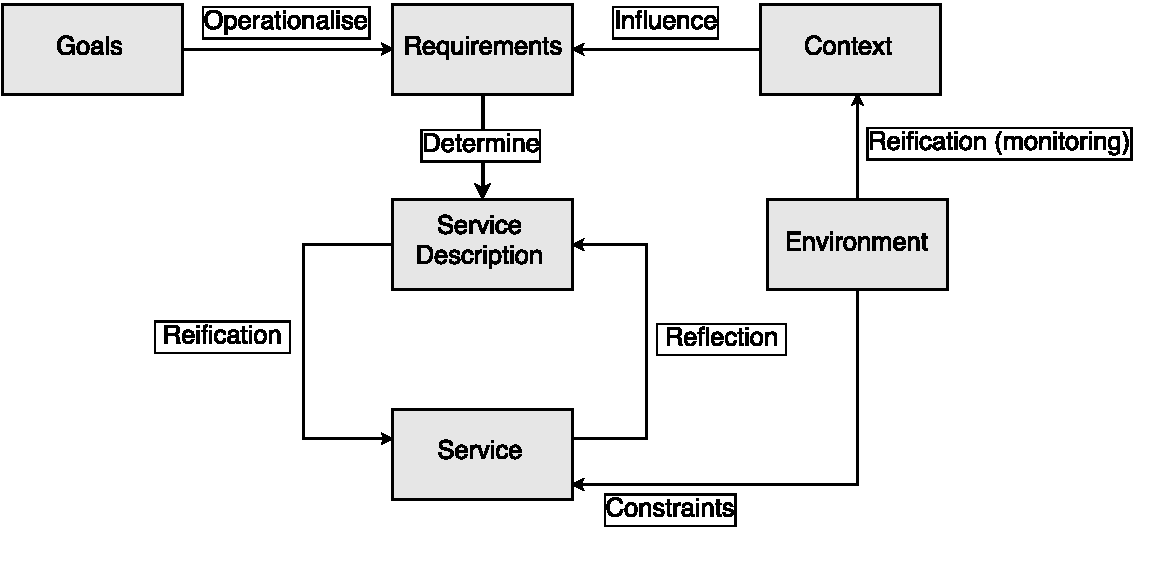
\includegraphics[width=.8\linewidth]{finkelstein_framework}
  \caption{Context-aware services framework by~\cite{finkelstein_framework_2001}}
\label{fig:finkelstein_framework}
\end{figure}

\emph{Environment} is whatever in the world provides a surrounding in which the agent is supposed to operate. The environment comprises such things as characteristics of the device that the agent is expected to operate in.
\emph{Context} is the reification of the environment. The \emph{context} provides a manageable, easily computer manipulable description of the \emph{environment}. A context-aware system should watch relevant environment properties and keep a runtime model that represents those properties. By reasoning about that model the system can change its behavior. A \emph{context} can be either an \emph{activator} of goals or a \emph{precondition} on the applicability of a certain strategy to reach a \emph{goal}.

A \emph{goal} is an objective the system should achieve. It is an abstract and long-term objective of the system. A \emph{requirement} operationalises a goal. It represents a more concrete and short-term objective that is directly achievable through actions performed by one or more agents. \emph{Service description} is the meta-level representation of the actual, real-world service. It should be a suitable formalism that allows services to be compared to requirements in order to identify runtime violations. Service provides the actual behavior as perceived by the user.

A \emph{reflective system} is a system which incorporates structures representing (aspects of) itself. A \emph{causal connection} between a model and a modeled element exists if one of them changes, this leads to a corresponding effect upon the other~\cite{maes_concepts_1987}. Following this approach, the system should keep a causal connection between the service and the description. The system adapts by manipulating the service description.
Following the requirements reflection vision~\cite{bencomo_requirements_2010}, a system should keep software requirements model at runtime, and use such model to drive the system adaptation.

%\input{parts/background/self-}
\section{Software Components}
Heineman define \emph{software component} as a
\say{software element that conforms to a component model and can be independently deployed and composed without modification according to a composition standard}\cite{heineman_component-based_2001}.

Software components is a unit of composition. Software systems are built by composing different components.  Software components must conform to a component model by having contractually specified interfaces and explicit context dependencies only.\cite{szyperski_component_2002}.

A \emph{component	interface} \say{defines a set of component functional properties, that is, a set of actions understood by both the interface provider (the component) and user (other components, or other software that interacts with the provider)}\cite{crnkovic_software_2011}.
A component interface has a role as a component specification and also a means for interaction between the component and its environment.
A \emph{component model} is a set of standards for a component implementation. These standards can standardize naming, interoperability, customization, composition, evolution and deployment.\cite{heineman_component-based_2001}
The \emph{component deployment} is the process that enables component integration into the system. A deployed component is registered in the system and ready to provide services\cite{crnkovic_software_2011}.
\emph{Component binding} is the process that connects different components through their interfaces and interaction channels.

Software architecture deals with the definition of components, their external behavior, and how they interact\cite{kaur_component_2010}. The architectural view of a software can be formalized via an architecture description language (ADL)\cite{medvidovic_classification_2000}.


Component-based software engineering (CBSE) approach consists of building systems from components as reusable units and keeping component development separate from system development\cite{crnkovic_software_2011}.

CBSE is built on the following four principles\cite{crnkovic_software_2011}:
\begin{itemize}
  \item \emph{Reusability}. Components, developed once, have the potential for reuse many times in different applications.
  \item \emph{Substitutability}. Systems maintain correctness even when one component replaces another.
  \item \emph{Extensibility}. Extensibility aims to support evolution by adding new components or evolving existing ones to extend the system’s functionality.
  \item \emph{Composability}. A system should support the composition of functional properties (component binding). Composition of extra functional properties, for example, composition of components’ reliability, is another possible form of composition.
\end{itemize}

\subsection{Component-Based Adaptation}

In the literature was proposed frameworks for architecture and components based adaptation.

Rainbow\cite{garlan_rainbow:_2004} is a framework for self-adaptation architecture based. It keeps an model of the architecture of the system and can be extended with rules to analysis the system behavior at runtime, find adaptation strategies and perform this changes. It separate the functional code (internal mechanisms) from adaptation code (external mechanism) in a schema called external control, influenced by control theory.

MUSIC\cite{rouvoy_music:_2009} project provides a component-based middleware for adaptation that propose to separate the self-adaptation from business logic and delegate adaptation logic to generic middleware. As in our propose it adapts by evaluating in runtime the utility of alternatives, to chose a feasible one (e.g., the one evaluated as with highest utility).

Flashmob~\cite{sykes_flashmob:_2011} is an approach for distributed self-assembly. Different from MUSIC and Rainbow, it handles component-based adaptation in a distributed environment. The self-assembly can be described as: given a set of available components (with various functional and non-functional properties), and a configuration of components which are already running, find a new configuration which works (better) in the changed execution environment (including hardware),
meets new user requirements or takes account of new component implementations~\cite{sykes_flashmob:_2011}. Flashmod uses a three-layer model: goals, management and components proposed by Kramer and Magee~\cite{kramer_self-managed_2007}, extending it to allow distributed agreement in a given configuration.

OSGi\cite{the_osgi_alliance_osgi_2007} is a Java centric platform that allows dynamic bind and unbind of components, usually named bundles. Ferreira et al.\cite{ferreira_-osgi:_2012} proposed a framework for adaptation based on OSGi.

\subsection{From Goals to Components}

Lamsweerde \cite{van_lamsweerde_system_2003} present a method for derive architecture from KAOS goal model. First an abstract draft is generated from functional goals. Secondly, the architecture is refined to meet non-functional requirements such as cohesion.

% Penserini \citep{penserini_design_2007} propose a method for generate agents from goal models.
% Morandini \cite{morandini_towards_2008}
% Tropos - Jadex-BDI}
Pimentel et al. \cite{pimentel_deriving_2012} present a method  using i* models to produce architectural models in Acme. If focus in he development of adaptive systems. First, it transforms a i* model into a modular i* model by means of horizontal transformation. Secondly, it creates an architecture model from the i* modularized model by means of vertical transformation. Architectural design models is made easier by the
presence of actor and dependency concepts.

Yu et al.~\cite{yu_goals_2008} proposed an approach for keep the variability that exists in the goal model into the architecture.
It present a method for creating a component-connector view from a goal model.
A preliminary component-connector view is generated from a goal model by creating an interface type for each goal. The interface name is directed derived from the goal name. Goals refinements result in implementation of components.
If a goal is And-decomposed, the component has as many \emph{requires} interfaces as subgoals.

\begin{lstlisting}
Component G {
  provides IG;
  requires IG1, IG2;
}
\end{lstlisting}

If the goal is OR-decomposed, the interface type of subgoals are the interface type of the parent goal.
%It's the most important patterns as it allow variability at architecture.

\begin{lstlisting}
Component G1 {
  provides IG;
}

Component G2 {
  provides IG;
}
\end{lstlisting}

A component equivalent to the parent goal is generated with a switch.


%TODO Input and outputs are added to the interface.

%TODO Related lower level components can be merged by parametrization.

\subsubsection{Dependency Injection}

Dependency Injection is a pattern that allow for wiring together software components that was developed without the knowledge about it other.~\cite{fowler_inversion_2004}

In OO languages normally you instantiate an Object from a class using an operator (\emph{new} for Java) and a reference to this class. By this the object that is instantiating (the object client) is dependent of the referenced class (the service implementation class). In case of strong typed languages, normally one will get an exception if the referenced class is not present.

So the use of the \emph{new} operator lead to the following disadvantages:
\begin{itemize}
  \item impose compile time dependency between two classes
  \item impose runtime dependency between two classes
\end{itemize}

The basic idea of the Dependency Injection, is to have a separate object, an assembler, that wire together the components at runtime\cite{fowler_inversion_2004}. The client class refer to service using its Interface (the service interface). The assembler can use alternative ways of the \emph{new} to instantiating an object, so that the wiring between client objects and implementation service classes could be postpone to runtime.

By this is we can at runtime:
\begin{itemize}
  \item discover available implementation of a service interface
  \item decide this implementation to instantiate from available implementations
\end{itemize}

Not always this pattern is needed as not always is useful to avoid the reference to a class. But in the context of component-based adaptation it would be specially useful to the decouple client components from service components, allowing runtime reasoning about what implementation to choose.

\begin{figure}[h!]\centering

\begin{tikzpicture}
  \begin{umlpackage}[x=4,y=0]{service interface}
    \umlemptyclass[width=15ex]{IServiceA}
  \end{umlpackage}
  \begin{umlpackage}[x=4,y=-3]{service implementation}
    \umlemptyclass[width=15ex]{ServiceAImpl}
    \umlimpl{ServiceAImpl}{IServiceA}
  \end{umlpackage}
  \begin{umlpackage}[x=0,y=0]{Client}
    \umlemptyclass[width=15ex]{ClientOfServiceA}
    \umlassoc{ClientOfServiceA}{IServiceA}
  \end{umlpackage}
  \begin{umlpackage}[x=0,y=-3]{Assembler}
  \end{umlpackage}
\end{tikzpicture}

\caption{Two components}
\end{figure}

% \subsubsection{Inversion of Control Containers}
% \label{sec:iocc}
%
% It have been used as a core principle in the development of popular frameworks like Sprint and Angular.

\subsection{Development of Self-Adaptive Systems}

For self-adaptive systems (SAS) some activities that traditionally occur at development-time are moved to runtime.  In\cite{andersson_software_2013}
was proposed a process for development of adaptive systems.
Activities performed externally are referred as \emph{off-line activities}, and activities performed internally as \emph{on-line activities}.

The right-hand side of Figure~\ref{fig:sas_lifecycle} depicts a running SAS. At this system we have \emph{Domain Logic} that solves that is responsible for final user goals achievements. And also, \emph{Adaptation Logic}, that is responsible to adapt the system in response to changes in the environment. Adaptation logic implements a control loop in line with the monitor-analyze-plan-execute (MAPE) loop~\cite{kephart_vision_2003}.

The left-hand side of Figure~\ref{fig:sas_lifecycle} represents a staged life-cycle model. Off-line activities work on artifacts such as design model and source code in a product repository and not directly on the running system.


\begin{figure}[!htb]
  \centering
  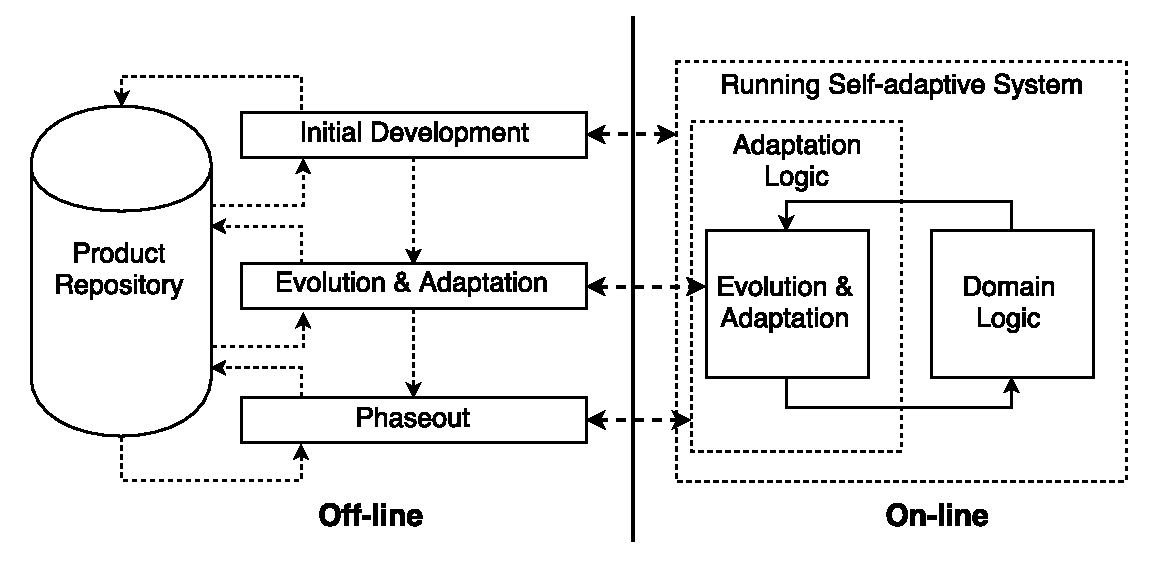
\includegraphics[width=\linewidth]{sas_lifecycle}
  \caption{A Life-cycle model for Self-Adaptation Software System\cite{andersson_software_2013}}
  \label{fig:sas_lifecycle}
\end{figure}

\subsection{Software Deployment}

Software deployment refers to all activities that make a software system available for use\cite{carzaniga_characterization_1998}. These activities result
in the creation and distribution of artifacts,  from the development environment to the target runtime environment. Artifacts are files that package software components and assets. The deployment process can vary depending on the application domain and execution platform. In embedded platforms, the deployment can consist in burning software into a chip. In consumers' personal or business domain, for a desktop platform, the deployment can consist of an installation process with collaboration between a person and a script that automates some steps.
In an enterprise domain, for a web platform it can consist in coping and editing some files in a couple of machines. In many of those scenarios software will be periodically updated, frequently becoming unavailable during the update process.
The complexity of the software deployment can also vary as a function of how much the platform is distributed (i.e. the number of nodes), how much heterogeneous it is, and how much is known about the deployment computing environment at design-time. In a dynamic and heterogeneous environment deployment can be specially complex.

\label{sub:deployment}
\begin{figure}[!htb]
  \centering
  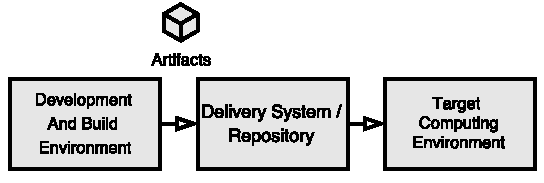
\includegraphics[width=.7\linewidth]{deployment_extended_process}
  \caption{Artifacts Deployment}
  \label{fig:deployment_extended_process}
\end{figure}

Deployment artifacts are the artifacts needed at the deployment environment. Artifacts are built at development and build environment. Built artifacts are move for a delivery system where they can be accessed from the target environment. At deployment the artifacts are moved from the delivery system to the target computing environment. Also, configuration activities can be realized.
In the software industry, a \emph{continuous integration}\cite{humble_continuous_2010} environment applies automation in building and getting components ready to delivery. In such environment if a developer pushes changes to a code repository, components are automatically built and published to delivery system. The build process commonly involves fetching build dependencies, compiling source code, running automated quality control (tests and static analysis) and packaging components into artifacts. Artifacts are published if target quality policies are met.
%dependency manager
Fundamental to continuous integration environments are \emph{Package Management Systems} tools, such as Maven\cite{apache_apache_2016} for Java platform. These tools simplify the management of software dependencies~\cite{spinellis_package_2012}. Such tools ensure that development team members are working with same dependencies that are used in the build environment.
%Sistemas de Gereencia de Pacotes simplificam o processo de instalacao de dependencias. Um pacote contem em um formato padronizado codigo ou codigo compilado, juntamente a sua documentacao e metadados [7]. Os metadados normalmente incluem nome, versao e especificacao de instalacao. Sistemas de Gerencia de Pacotes gerenciam a obtencao e instalac ̧a  ̃ o de dependˆ encias de forma automatizada, com o m ́ınimo de interac ̧ a  ̃o com o usu ́ ario e consequentemente favorecem a reprodutibilidade.
%build manager

Research in software configuration and deployment, has focused on responding to dynamisms in a known environment. This could be costs and failures in a cloud environmet \cite{ferreira_leite_user_2014}, changes in managed resources \citep{gunalp_rondo_2015}, and changes in the context of operation~\cite{bencomo_dynamically_2008}.

\emph{Continuous delivery}\cite{humble_continuous_2010} extends the continuous integration environment, moving components from the delivery system to a target computing environment with none or minimum human intervention.

In the industry, package managers such as aptitute/apt-get(Debian based Linux distributions)\cite{aoki_debian_2016}, yum (Red Hat based Linux distributions)\cite{svistunov_red_2016}, Homebrew (MacOS)\cite{homebrew_homebrew_2016} and Chocolatey (Windows)\cite{chocolatey_chocolatey_2016} are capable of solving dependencies and deploying software. They require that a managed application declare their dependencies by name and version. DevOps\cite{bang_grounded_2013} is a movement in software industry that advocates that all configuration steps needed to configure the computing environment should be written as code (\emph{infrastructure as code}), following best practices of software development. That movement favors the documentation, reproducibility, automation and scalability.
%Tools such as Puppet and Chef are used by devopers to manage infrastructure.
DevOps allows for management of scalable computing environments. It can offer a significant advantage for enterprise environment in relation to manual approaches in which system administrators configure the system by manually following configuration steps. Current continuous integration/delivery and DevOps practices are not sufficient for highly dynamic and heterogeneous target computing environments; they require that highly specialized system administrators to analyze the environment and create environment configuration descriptors.
%% Deployment in IoT??


\section{Multiagent systems (MAS)}
Wooldridge~\cite{woolridge_introduction_2001} defines Multiagent Systems (MAS) as systems composed of multiple interacting computing elements known as \emph{agents}.
Agents are computer systems that are capable of autonomous action and interacting with other agents.

\section{Dependability}
Dependability can be defined as the ability of a system to avoid faults in its services
that (1) are more frequent or (2) more severe than acceptable. Or as the characteristic of a system to be justifiably trusted.

A common terminology used for system deviations is the following: \cite{avizienis_basic_2004}

\begin{itemize}
  \item \textbf{failure}: (or \textif{service failure}) is a perceived deviation from the correct service provided by a system.
  \item \textbf{error}: is a deviation of correct internal system state that can lead to its subsequent failure.
  \item \textbf{fault}: is the adjudged or
hypothesized cause of an error
\end{itemize}

Dependability includes the following attributes:\cite{avizienis_basic_2004}
\begin{itemize}
  \item \textbf{availability}: readiness for correct service.
  \item \textbf{reliability}: continuity of correct service.
  \item \textbf{safety}: absence of catastrophic consequences on the
user(s) and the environment.
  \item \textbf{integrity}: absence of improper system alterations.
  \item \textbf{maintainability}: ability to undergo modifications and repairs.
\end{itemize}

Many means have been developed of how to attain the attributes of dependability. These means can be classified as:

\begin{itemize}
  \item \textbf{Fault prevention} means to prevent the occurrence or introduction of faults.
  \item \textbf{Fault tolerance} means to avoid service failures in the presence of faults.
  \item \textbf{Fault removal} means to reduce the number and severity of faults.
  \item \textbf{Fault forecasting} means to estimate the present number, the future incidence, and the likely consequences of faults.
\end{itemize}


% Erica Jen defines evolvability as an entity’s ability to “alter their structure or function so as to adapt to changing circumstances”
%robustness: Feature persistence under specified and unforeseen perturbations, obtained by switching among multiple strategic options such that those changes are dynamically tolerated.


\textif{Resilient systems} \cite{laprie_dependability_2008} are expected to continuously provide justifiably be trusted services despite changes coming from the environment or from their specifications.


\section{Attain Dependability at Runtime }
To keep dependability in face of uncertainty in the deployment environment some techniques have been proposed for runtime analysis at runtime.

% TODO you need to refer to other work related to dependability at runtime: antonio filieri work, QoSA, Salehie, Sam Malek. Not only the work we develop!

Felipe et al\cite{guimaraes_framework_2013} propose a method of fault-tolerance for a scientific workflow execution in grid.

Alessandro Leite \cite{ferreira_leite_user_2014} propose a fault tolerance schema for cloud deployment based on which a fault instance in the cloud is monitored and in case of failure the instance can be restarted or terminated and them a new instance created.

Danilo et al\cite{mendonca_dependability_2015} propose a methodology for fault forecasting by which developer, at design-time, annotate the goal decomposition in goal model and specify context variables. A special tool generate a formula for, given a context, evaluate the probability of achieve a goal at runtime.

% TODO Pessoa et al \cite{pessoa_dependable_2015} propose a ... with and evaluate it with focus on safety ...


 % reduce redundancy

%\section{Self-Adaptive Systems}


Self-adaptive systems have been accepted as a promising approach to tackle context change. Self-adaptivesses is an approach in which the system
\textit{"evaluates its own behavior and changes behavior when the evaluation indicates that it is not accomplishing what the software is intended to do, or when better functionality or performance is possible."}\cite{laddaga_self_1997}.

%kramer et al. dream

Self-adaptive software aims to adjust various artifacts or attributes in response to changes in the self and in the context of a software system\cite{salehie_self-adaptive_2009}.

A key concept in self-adaptive systems is the awareness of the system. It has two aspects\cite{salehie_self-adaptive_2009}:
\begin{itemize}
   \item \textit{self-awareness} means a system is aware of its own states and behaviors.
   \item \textit{context-awareness} means that the system is aware of its context,
\end{itemize}

Schilit et al.\cite{klein_survey_2008} define \textit{context} as \say{the sufficiently exact characterization of the situations of a system by means of perceivable information that is relevant for the adaptation of the system}.

Schilit et al.\cite{klein_survey_2008} define \textit{context adaptation} as \say{a system’s capability of gathering information about the domain it shares an interface with, evaluating this information and changing its observable behavior according to the current situation}.


% laddaga1997: it should relies on software informed about its mission and about its construction and behavior.  This implies that the software has multiple ways of accomplishing its purpose, and has enough knowledge of its construction to make effective changes at runtime.

% Such software should include functionality for evaluating its behavior and performance, and the ability to replan and reconfigure its operations in order to improve its operation.  Self adaptive software should also include a set of components for each major function, along with descriptions of the components, so that components of systems can be selected and scheduled at runtime, in response to the evaluators.

% It also requires the ability to impedance match input/output of sequenced components, and the ability to generate some of this code from specifications. In addition, we seek this new basis of adaptation to be applied at runtime, as opposed to development/design time, or as a maintenance activity.


% mape-k

% different approaches ref salehie

% challenges

%
% A self-managed software architecture is one in which components automatically configure their interaction in a way that is compatible with an overall architectural specification and achieves the goals of the system\cite{kramer_self-managed_2007}.

% Component Control
% include the capability to support component creation, deletion and interconnection.

% include facilities to report the current status of components to higher layers and also include the capability to support component creation, deletion and interconnection.
% adjust the operating parameters of components
% self-tuning algorithms, event and status reporting to higher levels and operations to support modification – component addition, deletion and interconnection.
% situation is met that the current configuration of components is not designed to deal with, this layer detects this failure and reports it to higher layers.



% Change Management

% Goal Management

%\section{Software Components and Architecture}

Heineman define \textit{software component} as a
\say{software element that conforms to a component model and can be independently deployed and composed without modification according to a composition standard}\cite{heineman_component-based_2001}.

Software components is a unit of composition. Software systems are build by composing different components.  Software components must conform to a component model by having contractually specified interfaces and explicit context dependencies only.\cite{szyperski_component_2002}.

A \textit{component	interface} \say{defines a set of component functional properties, that is, a set of actions that’s understood by both the interface provider (the component) and user (other components, or other software that interacts with the provider)}\cite{crnkovic_software_2011}.
A component interface has a role as a component specification and also a means for interaction between the component and its environment.
A \textit{component model} is a set of standards for a component implementation. These standards can standardize naming, interoperability, customization, composition, evolution and deployment.\cite{heineman_component-based_2001}

The \textit{component deployment} is the process that enables component integration into the system. A deployed component is registered in the system and ready to provide services \cite{crnkovic_software_2011}.

\textit{Component Binding} is the process that connects different components through their interfaces and interaction channels.

Software architecture deals with the definition of components, their external behavior, and how they interact.\cite{kaur_component_2010}

Component based software engineering (CBSE) approach consists in building systems from components as reusable units and keeping component development separate from system development\cite{crnkovic_software_2011}.

CBSE is built on the following four principles\cite{crnkovic_software_2011}:
\begin{itemize}
  \item Reusability. Components, developed once, have the potential for reuse many times in different applications.
  \item Substitutability. Systems maintain correctness even when one component replaces another.
  \item Extensibility. Extensibility aims to support evolution by adding new components or evolving existing ones to extend the system’s functionality.
  \item Composability. System should supports the composition of functional properties (component binding). Composition of extra functional properties, for example composition of components’ reliability, is another possible form of composition.
\end{itemize}

%\section{Goal-oriented requirements engineering}

Goal-oriented requirements engineering (GORE) is concerned with the use of goals for eliciting, elaborating, structuring, specifying, analyzing, negotiating, documenting, and modifying requirements\cite{van_lamsweerde_goal-oriented_2001}.

GORE models are the main tool used by system analysts and stakeholders to reason about the system requirements. Goal modeling represents a shift in relation to traditional software development approaches as it focus on stakeholder goals and states that the system needs to achieve and not in how it achieves it\cite{ali_goal-based_2010}. Goal models are graphs representing AND/OR-decomposition of abstract goals down to operationalisable leaf-level goals. \cite{morandini_operational_2009}

A goal is an objective the system under consideration should achieve. \cite{van_lamsweerde_goal-oriented_2001}

\section{TROPOS}
Tropos\cite{bresciani_tropos:_2004} is a methodology for develop multi-agent systems that uses goal models for requirement analyses. Tropos encompasses the software development phases, from Early Requirements to Implementation and Testing.

\subsection{The Tropos key concepts}

The methodology adopts the i* \cite{yu_modelling_1996} modeling framework, which proposes the concepts of actor, goal, task, resource and social dependency to model both the system-to-be and its organizational operating environment\cite{bresciani_tropos:_2004}. In more recent publication \cite{morandini_tropos_2014} about the Tropos modeling framework the concept of \textit{task} was renamed to \textit{plan}.

The following are the key concepts in the Tropos metamodel\cite{morandini_tropos_2014}:

\begin{itemize}
    \item Actor: an entity that has strategic goals and intentionality
    \item Goals: it represents actors’ strategic interests. \texit{Hard goals} are goals that have clear-cut criteria for deciding whether they are satisfied or not. \textit{Softgoals} have no clear-cut criteria and are normally used to describe preferences and quality-of-service demands.

    \item Plan: it represents, at an abstract level, a way of doing something. The execution of a plan can be a means for satisfying a goal or for \textit{satisficing} (i.e. sufficiently satisfying) a softgoal.

    \item Resource: it represents a physical or an informational entity.

    \item Dependency: its a relationship between to actors that specify that one actor (the \textif{depended}) have a dependency to other actor (the \textit{dependee}) to attain some goal, execute some plan or deliver a resource. The object of the dependence is the \texit{dependum}.

    \item Capability: it represents both the \textit{ability} of an actor to perform some action and the \textit{opportunity} of doing this.

\end{itemize}

% TODO Runtime goal models

%\section{Dependency Injection}

Dependency Injection is a patter that allow for wiring together software components that was developed without the knowledge about it other. \cite{fowler_inversion_2004}

In OO languages normally you instantiate an Object from a class using an operator (\textit{new} for Java ) and a reference to this class. By this the object that is instantiating (the object client) is dependent of the referenced class (the service implementation class). In case of strong typed languages, normally one will get an exception if the referenced class is not present.

So the use of the \textit{new} operator lead to the following disadvantages:
\begin{itemize}
  \item impose compile time dependency between two classes
  \item impose runtime dependency between two classes
\end{itemize}

The basic idea of the Dependency Injection, is to have a separate object, an assembler, that wire together the components at runtime\cite{fowler_inversion_2004}. The client class refer to service using its Interface (the service interface).

The assembler can use alternative ways of the \textit{new} to instantiating an object, so that the wiring between client objects and implementation service classes could be postpone to runtime.
By this is we can at runtime:
\begin{itemize}
  \item discover available implementation of a service interface
  \item decide this implementation to instantiate from available implementations
\end{itemize}

Not always this pattern is needed as not always is useful to avoid the reference to a class. But in the context of component-based adaptation it would be specially useful to the decouple client components from service components, allowing runtime reasoning about what implementation to choose.

\begin{figure}[h!]\centering

\begin{tikzpicture}
  \begin{umlpackage}[x=4,y=0]{service interface}
    \umlemptyclass[width=15ex]{IServiceA}
  \end{umlpackage}
\begin{umlpackage}[x=0,y=0]{service implementation}
  \umlemptyclass[width=15ex]{ServiceAImpl}
  \umlimpl{ServiceAImpl}{IServiceA}
\end{umlpackage}
\begin{umlpackage}[x=8,y=0]{Client}
  \umlemptyclass[width=15ex]{ClientOfServiceA}
  \umlassoc{ClientOfServiceA}{IServiceA}
\end{umlpackage}
\begin{umlpackage}[x=12,y=0]{Assembler}

\end{umlpackage}

\end{tikzpicture}

\caption{Two components}
\end{figure}

\section{Inversion of Control Containers}
\label{sec:iocc}

It have been used as a core principle in the development of popular frameworks like Sprint and Angular.


\chapter{Related Work}
\section{Related Work}
\label{sec:related}

In the literature, there are proposals that tackle the problem of handling changes at system context~\cite{angelopoulos_capturing_2015}\cite{knauss_acon:_2016}. These proposals focus on the system external context, reasoning about known facts about the external managed world and how it affects the systems goals.
Asadie et al.~\cite{asadi_goal-oriented_2011} relates Goal-Oriented requirements and feature models for the development of SPL using a goal-oriented approach. In the described approach Goal-Models complement feature-models providing a mechanism to choose a set of features from stakeholder intentions.
Angelopoulos et al.~\cite{angelopoulos_capturing_2015} present an approach to handle context variability at three different levels: goals, behavior and architecture.


Rainbow is a framework for self-adaptation architecture based\cite{garlan_rainbow:_2004}. It keeps an model of the architecture of the system and can be extended with rules to analysis the system behavior at runtime, find adaptation strategies and perform this changes. It separate the functional code (internal mechanisms) from adaptation code (external mechanism) in a schema called external control, influenced by control theory. \cite{garlan_software_2009}
%Different from our proposal Rainbow don't enforce an specific architecture what could be special useful in case of retrofitting a pre-existent systems.
Different from our proposal it isn't goal-oriented an there is no work on how to relate Rainbow components to requirements.

MUSIC project provides a component-based middleware for adaptation that propose to separate the self-adaptation from business logic and delegate adaptation logic to generic middleware. As in our propose it adapts by evaluating in runtime the utility of alternatives, to chose a feasible one (e.g., the one evaluated as with highest utility)\cite{rouvoy_music:_2009}. As Rainbow, MUSIC is not goal-oriented.
% Yet it provide means of supporting seamless configuration of component frameworks based on local, remote components and services.

Salehie et al. \cite{salehie_towards_2012} propose a run-time goal model and its related action selection. It models adaptable software as a system that exposes sensors and effectors and  proposes a model consisting in Goals, Attributes and Action for selecting actions that will effect the adaptable software at runtime, giving sensed attributes.
So the adaptation mechanism is to choose the best action given the actual attributes.
As this work it uses explicit runtime goals and make them visible and traceable.
Different from it we use a more symmetric approach that can allow for functional
and adaptation management.
%The validation is make on simulated environment.

Günalp et al. \cite{gunalp_autonomic_2012}\citep{gunalp_rondo_2015} propose a middleware for pervasive software with autonomic capabilities. The approach is service based. It proposes a component written in a custom language and the use of components repository that allows the discovery on new sensors. The system present a support for adaptability by using policies.
% Different from this work it did not present support for collaboration/delegation of goals to another peers. It don't allow for runtime incorporation of adaptation strategies, also.

%% Traceability
Pinto et al. \cite{pinto_process_2005} introduces a approach to support traceability through requirements specifications, system architecture models, static and dynamic software design models and implementation artifacts of agent-oriented software systems.
The authors use a set of types of relationships and structure the traceable information in levels (external, organizational and management) to improve the semantic of requirement traceability.
The work also includes a process to be followed during the development of the traceability model

\cite{bencomo_dynamically_2008} uses a SPL approach. It associate a architecture variability model with a environment variability model. The environment variability is modeled as a transition system. The structural variability is responsible for the system adaptation. A configuration or a product is a set of component selected. A configuration is associated with states in the environment variability model. It focus on the adaptation in the configuration at runtime but not in the deployment. The variability model as presented do not allow for open adaptation. Mizouni at al. \citep{mizouni_framework_2014} uses a feature model associated with context requirements.

Ali et~al.\cite{ali_requirements-driven_2014} explore the optimization of the deployment for a given context variability space in which the system will be deployed. It differ from this work in which we explore the variability in the computing environment itself, in terms of computing resources available to the system. We envisage that a joint usage with our approach would enrich the adaptiveness to the system to a a given environment.

% GOAL-Architecture
In this work we present a Goal-Architecture view. Such view was presented in the literature. STREAM-A\cite{pimentel_deriving_2012} create specialized agents. We create components. Components are not agents as they do not have autonomy, instead they are means of achieving a goal.

% But must of these approaches ignores variability in the computing environment, the underline computing resources that form the infrastructure for executing the system software. None of them solve the problem of software development for a highly variable environment from different software providers. Our approach focus on how move components to target environment.

Leite et al. \cite{ferreira_leite_user_2014} proposes and approach for automatic deployment on inter-cloud environments. It relies on abstract and concrete features models and constraint satisfaction problem solver to create a computing environment using resources distributes across various clouds. The approach relies on centralized models of the environment and not address open adaptation problem.

% While package mangers such as aptitude and RPM can get components and handle some variabilities, e.g CPU architecture, they are not adaptive, so they not handle changes in the computing environment at runtime. They favor reuse at a library level. We propose reuse at component level.

Table~\ref{table_related_works} characterizes and compares research related to Goald.

\begin{table*}[]
\centering
\caption{Comparing characteristic properties of selected approaches related to Goald}
\label{table_related_works}
\begin{tabular}{|l|l|l|l|l|}
\hline
 \textbf{Work by} & \textbf{Goal-oriented} & \textbf{Adaptive Deployment} &  \textbf{Open Adaptation} \\ \hline
Ali et al.\citep{ali_requirements-driven_2014} & Yes & No & No \\ \hline
Gunalp et al.\citep{gunalp_rondo_2015} & No & Yes  &  No\\ \hline
Leite et al. \citep{ferreira_leite_user_2014}  & No & Yes & No \\ \hline
Mizouni et al. \citep{mizouni_framework_2014} & No & Yes & No \\ \hline
Goald & Yes & Yes & Yes \\ \hline
\end{tabular}
\end{table*}


\chapter{Proposal}
% Proposal (3.5p)
\section{Proposed Method}
\label{sec:proposal}

% General discussion
An autonomous deployment platform should maximize the opportunity to make goals achievable by preparing the system for a broad range of context variability space.


This section describes our method to tackle the challenges presented in~(\ref{sec:challenges}). It consists in offline activities for development of artifacts keeping trace to user goals. And in online support to autonomous handle deployment.

As offline activities, components are defined from a CGM using appropriate patterns. These components are packaged in artifacts together with metadata that describe what goals the packaged component can achieve, its context restrictions and dependencies.

At runtime the adaptation platform receive what goals the user wants to achieve in that environment and look for artifacts that allows it achieve its goals. The platform them assemble and architecture that allows the goal achievement.

\begin{figure*}[!htb]
  \centering
  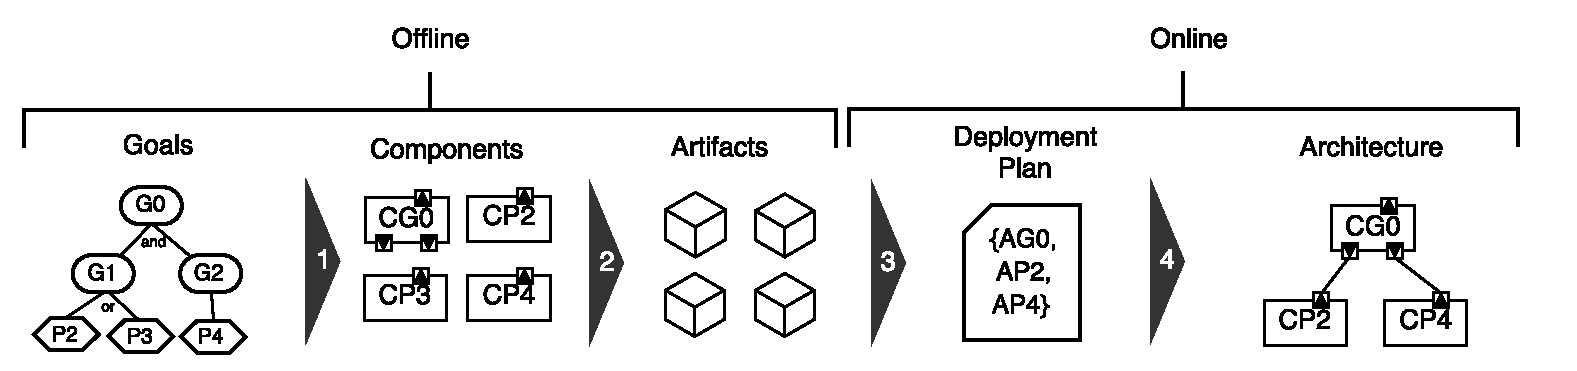
\includegraphics[width=0.8\linewidth]{transformations}
  \caption{Transformations: (1) components definition; (2) packaging; (3) deployment}
\label{fig:overview}
\end{figure*}


Relate Architecture with Requirements.

\begin{figure}[!htb]
  \centering
  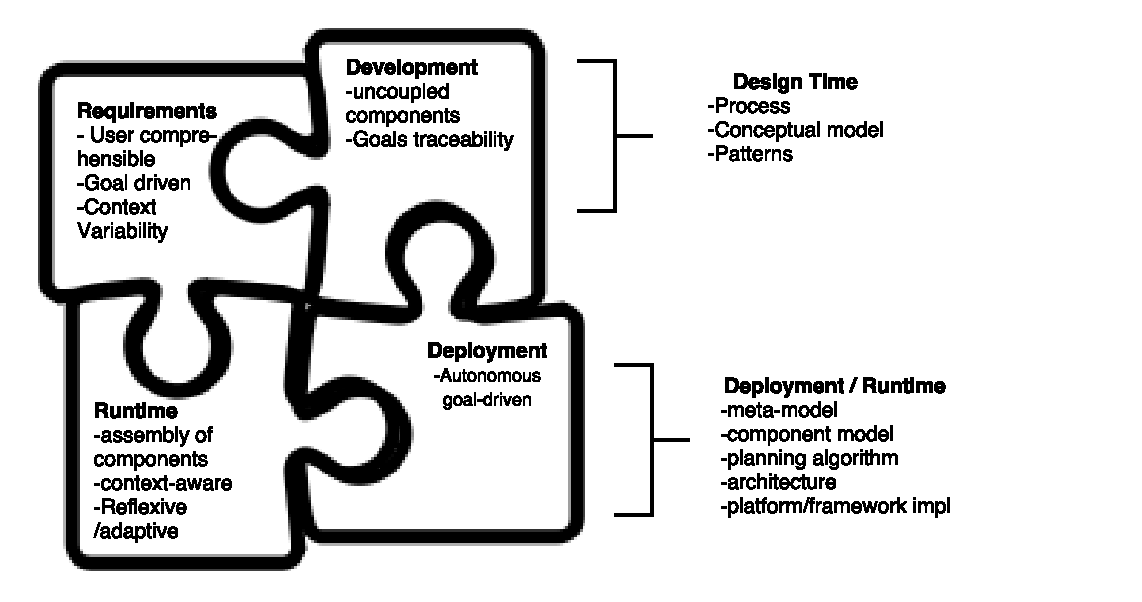
\includegraphics[width=\linewidth]{jig-saw}
  \caption{Proposal Overview}
\label{fig:overview}
\end{figure}



\subsection{Concepts}

\subsubsection{Context and Context Conditions}
\label{context}

In this work we are interested in conditions related with the computing environment. These conditions are related with availability of computing resources, e.g. take a game that can be rendered using CPU or GPU, the availability of GPU is a contextual condition that restrict the achievement of goal render game using GPU strategy.
Adopting the context model proposed in \cite{ali_goal-based_2010} we will express such conditions as formulae in a set of facts. A given context satisfy a context condition if all related facts are monitored and the formulae associated are true.

The facts can be of an atomic proposition such as GPU, that is evaluated to true if an associated resource are known to be available, and it is evaluated to false otherwise.
The facts can be also logical conditions using logical operators ==, !=, <, <=, >, >=.


\subsubsection{Goals, Components and Artifacts}
\label{sec:rules}

We enhance enhance component description with context condition. We extend Yu et al.\cite{yu_goals_2008} patterns for the Goals-Component view with contextual conditions.

\begin{table}[]
\centering
\caption{Contextual Goal Model to components; (1) context condition, (2) And-decomposition, (3)OR-decomposition}
\label{table_related_works}
\begin{tabular}{|l|l|}
\hline
 %\textbf{ A } & \textbf{ B} & \textbf{C} \\ \hline
 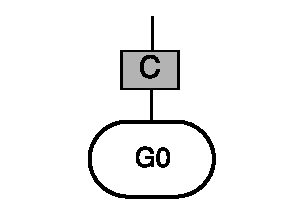
\includegraphics[scale=0.5]{patterns_condition} &
 \begin{lstlisting}
 Component G0 {
   provides IG0;
   condition C;
 }
 \end{lstlisting} \\ \hline
 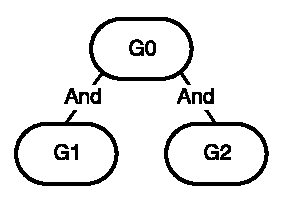
\includegraphics[scale=0.5]{patterns_and_decomposition} &
 \begin{lstlisting}
 Component G0 {
   provides IG0;
   requires IG1, IG2;
 }
 \end{lstlisting} \\ \hline
 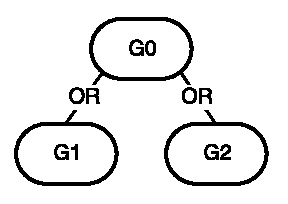
\includegraphics[scale=0.5]{patterns_or_decomposition} &
 \begin{lstlisting}
 Component G1 {
   provides IG0;
 }
 Component G2 {
   provides IG0;
 }
 \end{lstlisting} \\ \hline
\end{tabular}
\end{table}

Software component should be packaged in a standard packaging schema.
The package should, also, have meta-data describing goals it provides, context conditions, and dependencies.

Artifact is a tupla (component, metadata) and metadata is a tupla (context conditions, dependencies, provided goals) context, goals and dependencies.

\begin{itemize}
  \item Context conditions can be evaluated against the context. If the conditions are not satisfied the machine should not deploy the component.
  \item Dependencies are required services that should be provided by other components. Before deploy the component the machine should verify if it can satisfy the dependencies of the component.
  \item Provided goals are services that the component provide to the user or to other components.
\end{itemize}

The artifact dependency: all that its components depend
The artifact provide:  all that its components provide
The artifact conditions:  all that its components conditions

If both context conditions and dependencies are satisfied, the artifact is capable of allow the goal achievement.

\subsubsection{Online Goals}

In traditional goal modeling the agent have a root goal that are refined in subgoals.  Or-refinements allow for variability points in the goal model, but that refinement are static, at least for a given version of the goal model.
We argue that in a dynamic and open environment that vision is not sufficient. We propose a different vision for the autonomous deployment. An agent should have a set of goals that it should pursue. That set can be updated by and user or the agent itself when following a self-assembly approach~\cite{sykes_flashmob:_2011}. We call \emph{active goal} a goal that the agent must pursue.
In a dynamic environment, the agent can at a given moment have or not the resources to achieve a goal. \emph{Achievable Goal} is a goal that the agent pursue and is capable of achieve.

In our deployment view of the goals, we will consider a goal achievable if we can deploy at least one artifact that provide that goals.

\subsubsection{Evolution}

evolve without great effort.

We argue that a goal model can be seen as a protocol definition. When we create OR-Refinements we are giving alternatives of execution, creating variability points.

By creating interfaces in variability points
Open deployment platform.

  and we create opportunity for thirty-parties provide new alternativies

having different context condition will allow the goal to be achievable in a broader range of contexts: for example, in screen controls will allow the game to be playable at touch screen devices.

In tradition deployment schema, a complete new version of the software should be released.

\begin{figure}[!htb]
  \centering
  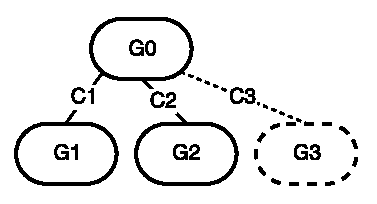
\includegraphics[width=\linewidth]{evolution_or}
  \caption{Evolution OR}
\label{fig:evolution_or}
\end{figure}

Component development and release

\subsubsection{Meta-model}

%TODO Research about goal driven adaptation terminonogy: nelly bencomo

\begin{figure}
  \centering
  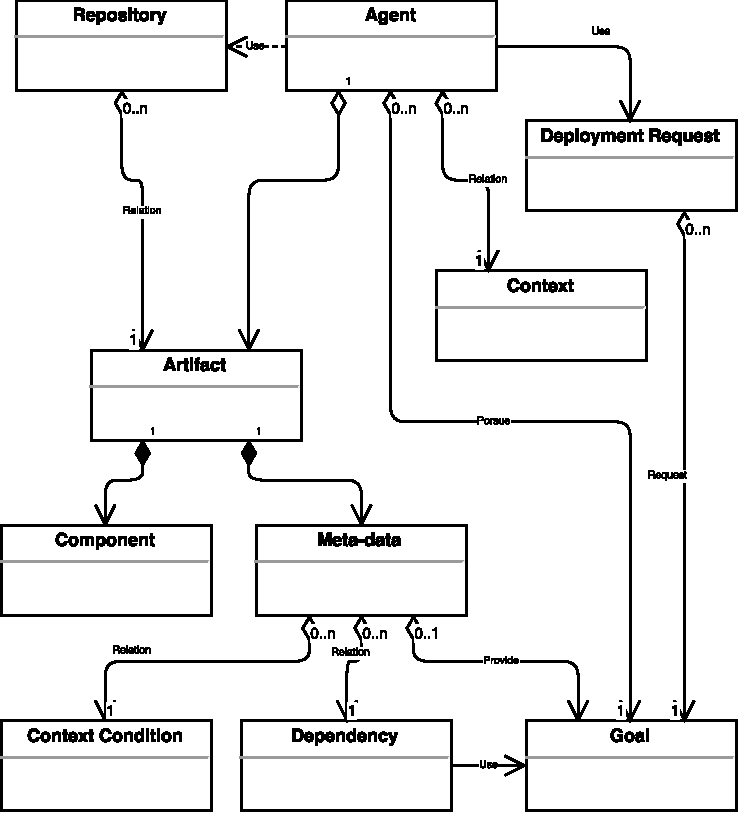
\includegraphics[width=0.8\linewidth]{meta-model}
  \caption{The Goalp Deployment meta-model}
  \label{fig:meta-model}
\end{figure}


\subsection{Off-line}
\label{sec:offline}
%
% The proposed approach is divides in two parts: first, we define a systematic way for a designer specify deployment restrictions to the goal model of the system. Each plan is associated with required computing environment context. We present a Tropos metamodel extension for specify computing environment resources and plans computing environment dependencies.
%
% Second, we introduce an approach for execute the deployment for a given computing environment. The deployment process here encompass deciding with computing resources will be responsible for executing each plan (respecting dependencies restrictions), and which operation needs to be executed in order to realize the deploymet.

%The complete deployment process is illustrated in figure \ref{fig:deployment_process_flow}.

\subsubsection{Roles}
The proposed process considers three roles: users, requirements engineers and software architects.
 Figure~\ref{fig:process_roles} summarize the collaboration between the roles.

\begin{description}
  \item[User]
  This role has access to a particular computing environment and want to achieve some goals there.
  \item[Requirements Engineer]
  Is responsible to translate users goals to a contextual goal model. Also is responsible to analyze the different contexts that the system is meant to operate and how it affects the goals.
  \item[Architect] Architect project the software architecture such as to permit variability of deployment.
  From the point of view of dynamic heterogeneous computing environments, the focus is to create interfaces for components that can allow for goal achievements using different computing resources.

\end{description}

\begin{figure}[!htb]
  \centering
  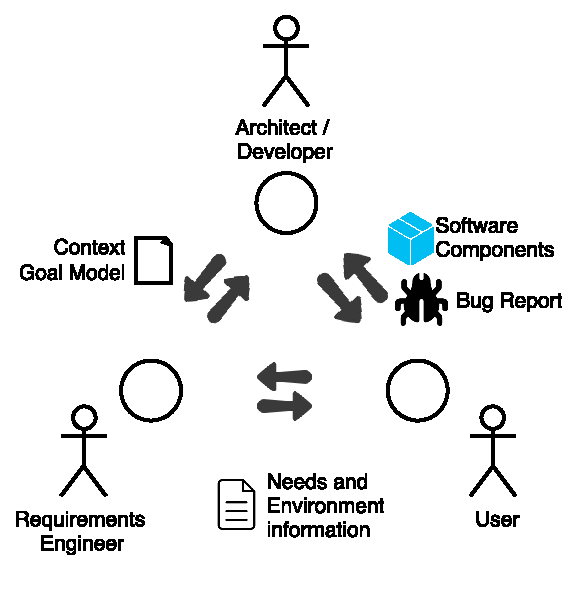
\includegraphics[width=.6\linewidth]{process_roles}
  \caption{Roles collaboration}
\label{fig:process_roles}
\end{figure}

\subsubsection{Activities}

Figure~\ref{fig:deployment_process_flow} describe the development process activities.

\label{sub:Proposal}
\begin{figure}[!htb]
  \centering
  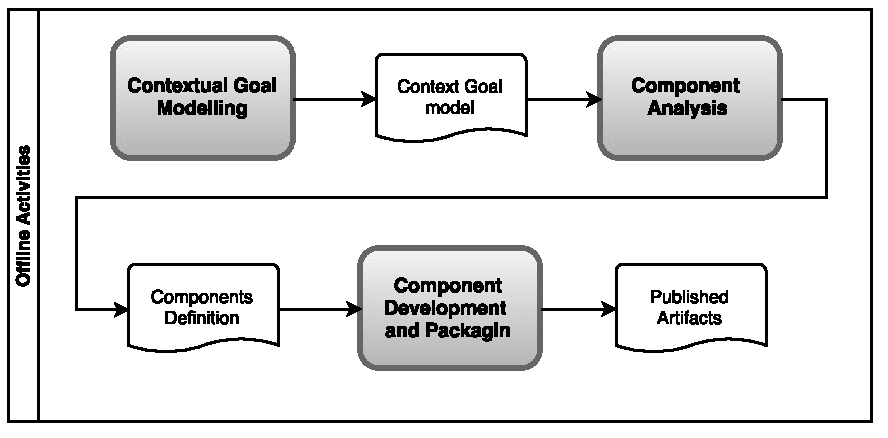
\includegraphics[width=\linewidth]{deployment_process_flow}
  \caption{Deployment Process Activities}
\label{fig:deployment_process_flow}
\end{figure}

\subsubsection{Goal Modeling}
This phase is coordinated by a requirement engineer with participation of a domain specialist, possibly the user.
A process such as TROPOS can be used. The output of this phase is a goal model.
Here, the goal model assumes a central role in the software development process. The goal model besides define the space of the solution, also works as common language. The goal model formalize the domain knowledge. It defines a common language between user and developers that will allow software deployment driven by user goals.


\subsubsection{Context Goal Modeling}
In this phase, the Goal model should be annotated with \emph{context conditions} related with the computing environment. That analysis is a context analysis and could benefit of the process described in~\cite{ali_goal-based_2010}. The requirements engineer should use knowledge about the computing resources that may be available at the computing environment.


\subsubsection{Component Analysis}
Software engineer should identify variability points.
Variability points in the contextual goal model are points where goals can be achieve with different strategies, each one having different context conditions.
Component interfaces are created following the guidelines described in Section~\ref{sec:rules}. The input and output of components are defined.

Also at this phase, it should be defined the sensors needed to evaluate facts about the computing environment.

\subsubsection{Component Development and Packaging}

Component development includes the cycle coding, build and test of software components.
The component package in the standard packaging schema is an artifact and should be put in a delivery system.


\subsubsection{Deployment Actors}

Repository


Node

Artifacts
Interfaces for RC4 open adaptation
Artifacts annotated with requirements and dependencies.


% TODO Relate the challenges with Deployment Manager features


Figure Respository-Platform-Request


\subsection{On-line}
\label{sec:online}


\subsubsection{Deployment Description}

Simple as possible to tackle RC5 (deployment specification accessible to users)


Goal
Subgoals

Mandatory Goals
Optional Goals


Example:
Bomberman

PlayBomberman
Mandatory:BombermanModel
BombermanVideo
BombermanControl
Optional:BombermanAudio

Repo:BombermanControlKeyboard, BombermanControlJoystick


\subsubsection{Goald}
\label{sec:goald}


\begin{figure}[!htb]
  \centering
  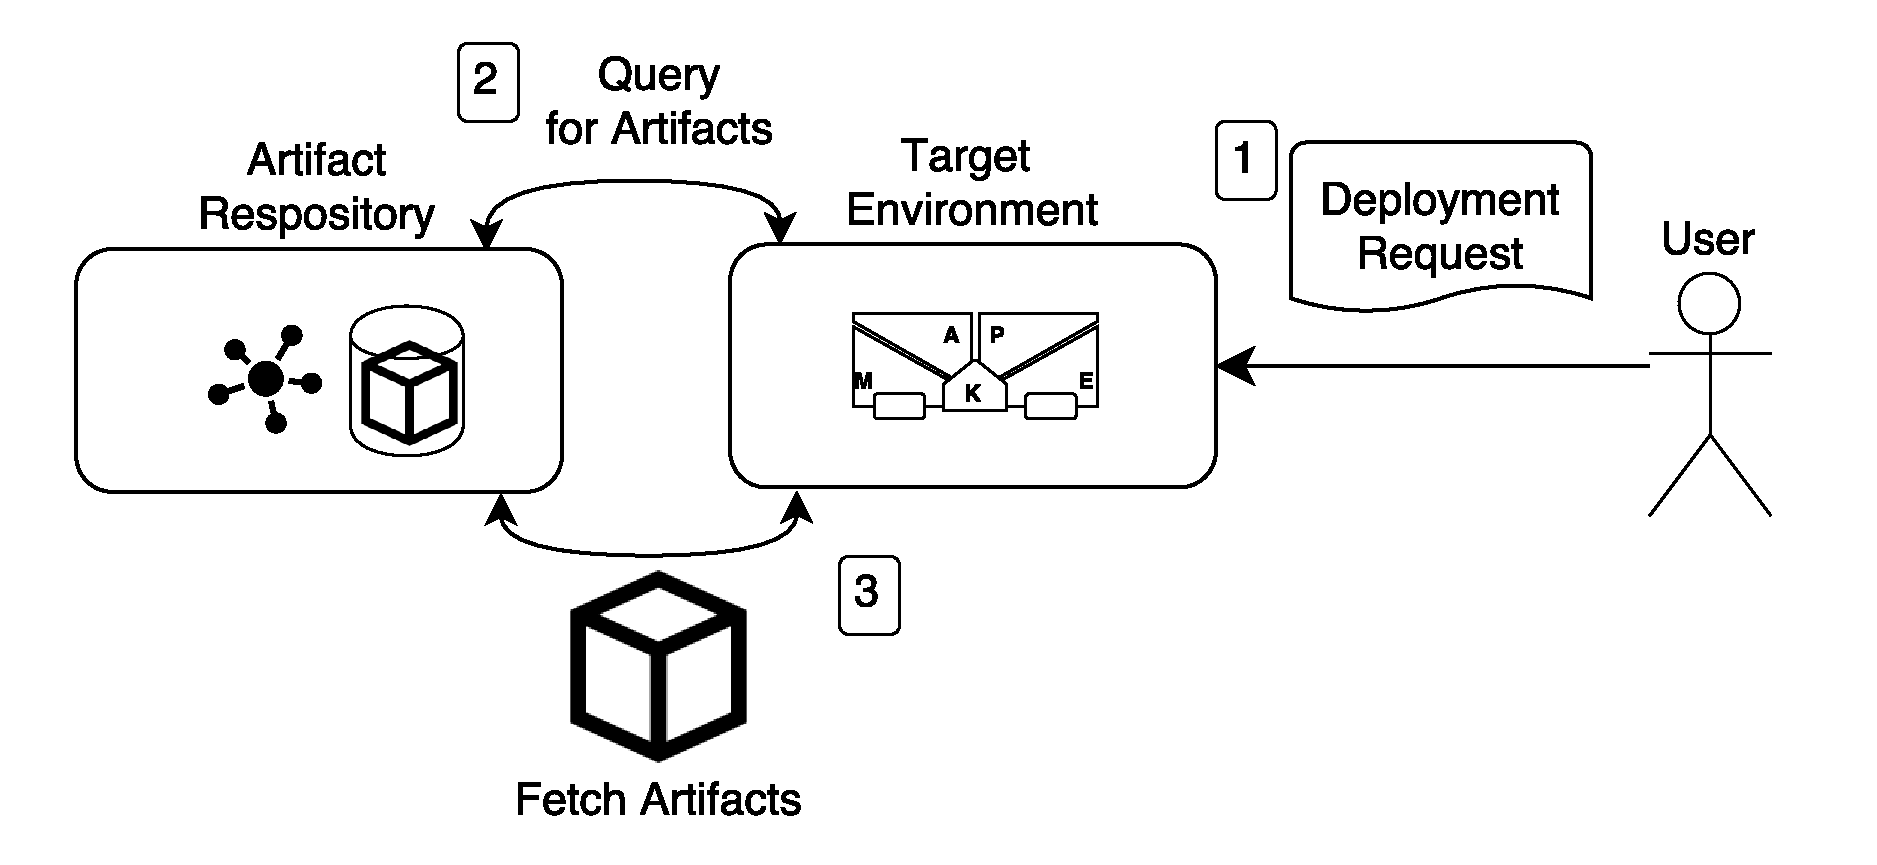
\includegraphics[width=\linewidth]{deployment_actors}
  \caption{Goald Deployment Actors}
\label{fig:deployment_actors}
\end{figure}

Figure~\ref{fig:deployment_actors} depicts the deployment execution. A user interested in using a computing environment to achieve a set of goals submits to this environment which goals it want to achieve in the form of a deployment request.

Then, our system introspect about available computing resources and artifacts present in repository and plan the deployment, generating a deployment plan that is a selection of artifacts that can allow for the goals achievement in the available computing environment. The deployment is them executed by fetching the appropriate artifacts from the repositories.

Facts about the computing environment are directed monitored by the agent by means of sensors. An Artifact should have in its meta-data the condition for its deployment. That condition is specified by a formula of facts.

\subsubsection{Deployment Manager}

Deployment Operations
install
uninstall

\subsubsection{Component Model}
\begin{itemize}
  \item Requirements
  \item Dependencies
\end{itemize}

\begin{itemize}
    \item Information it queries
    \item Listened Events
    \item Dispatched Events
    \item Periodic Execution
\end{itemize}


Life cycle

\begin{figure}[!htb]
  \centering
  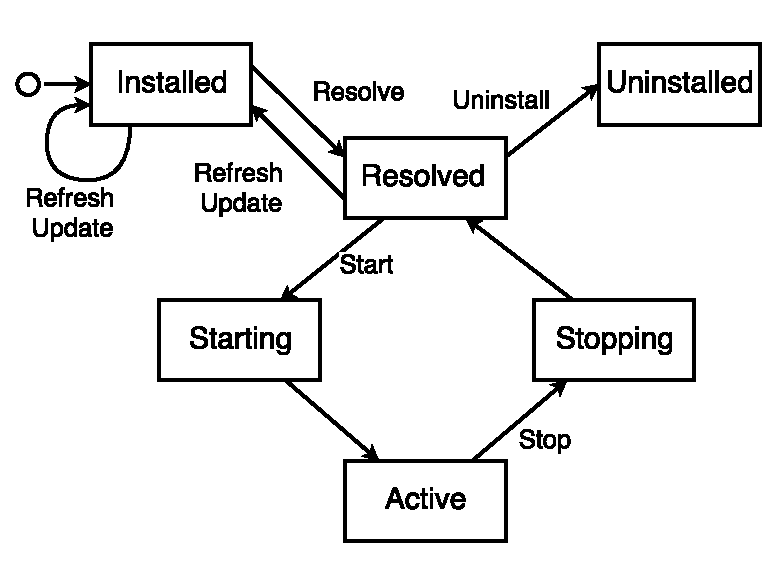
\includegraphics[width=.6\linewidth]{component_life_cycle}
  \caption{Component Life Cycle}
\label{fig:component_life_cycle}
\end{figure}


\begin{itemize}
  \item install
  \item register (listeners)
  \item uninstall
\end{itemize}

Dynamic binding

\subsubsection{Application}

Escalonando a aplicação e o código de adaptação.

\subsubsection{Initial Setup}

Knowledge base,
Component model of the platform: mape-k is in it self a component.



\subsubsection{Illustrative Scenarios}
New Goal

Adapt to resource failure


\subsubsection{Open Adaptation}

\subsubsection{Evolution 1: Notify user about not achievable goals}
If a goal is not achievable a event is generated. With this another component can take action such as notify a external agent (e.g a user) that a goal is not achievable locally with current resources and known components.


\subsubsection{Evolution 2: Adaptive monitoring policies}
% Monitoring policy
A monitor is associated with a monitoring policy that dictate the periodicy that the sense should occur.
\begin{itemize}
  \item periódico:
  \item on demand: Is executed in response to a query
  \item listener: Is called by another system component or external actor.
\end{itemize}



\subsubsection{Addressing Challenges}
RC1 uncertainty at design time and RC2 heterogeneous computing environment

We address these challenges by assembling the system at runtime driven by user goals. Using our approach the developer do not need to know the exact specification of the user environment.
We tackle challenge RC2 (heterogeneous computing environment) using decentralized approach to handle variability of computing environment.

RC3 dynamism
We address this challenge by providing an adaptation framework to handle changes in the computing environment.
Analyzing and responding to changes in the computing environment.

RC4 open adaptation
We address this challenge by providing descentralized approach based on interfaces so that third party developers can provide new components to the system at runtime.


RC5 deployment specification accessible to users
We address this by using goals as abstract way of specifying the system deployment. By this the user do not need to know details about system administration to configure a system. In our approach system administration rules and policies can be implemented as components.


\subsubsection{Architecture}

\begin{figure}[!htb]
  \centering
  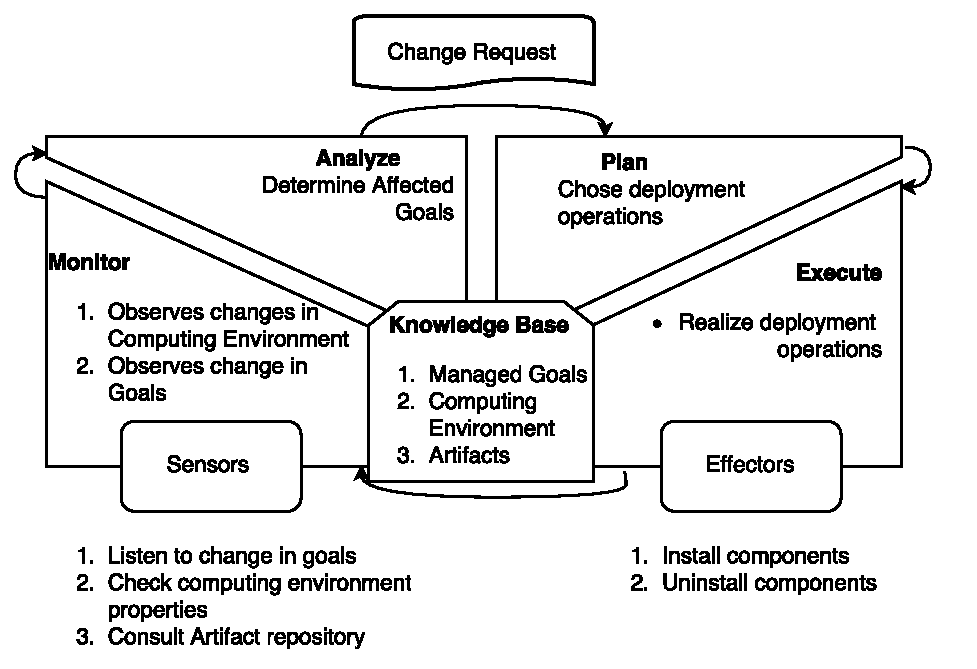
\includegraphics[width=\linewidth]{goald_mape_k}
  \caption{Goald Deployment Manager}
\label{fig:goald_mape_k}
\end{figure}

\begin{itemize}
  \item events: are handled to registered listeners.
\end{itemize}

\subsubsection{Knowledge Base}

The knowledge base store a model of goals the system much achieve, the computing environment context and current deployed artifacts.

The information in the knowledge base can be of two types:
\begin{itemize}
  \item facts: can be queried about by registered components
\end{itemize}


\subsubsection{Monitors}

Monitors are components that observes changes in the goals and context. All
\begin{itemize}
  \item Goal Change Monitor is responsible for listening to request of include or remove goals.
  \item Computing Environment monitor is responsible to verify \emph{facts} about the computing enivronment as introduced in~\ref{context}. \emph{Facts} are stored in the Knowledge Base and used to evaluate context conditions.
  \item Repository monitors observe changes in software repositories.
  \item Introspective monitors observe the system state and behavior. (ex: monitor that check if there is any monitor that dispatches events that no one cares about)
\end{itemize}

The result of monitors can be:
\begin{itemize}
  \item Change the knowledge base
  \item Dispatch Events
\end{itemize}

Core Components:
\begin{itemize}
  \item Timer Monitoring Policy:
  \item Computing Environment Sensors: listen to timeouts of monitoring policy. Sense the environment. Update the knowledge base and dispatch events for changes in the environment.
  \item Goals change listeners: listen for external entities that want to change the goals of the machine. The interface is implementation dependent (e.g HTTP service, GUI, command line). Dispatch External Change Requests.
  \item Repository Monitor: queries repository for information about components.
\end{itemize}



\subsubsection{Analyzer}

Objective change analyzer

Computing environment change - evaluate if any system goal is affected.

Evaluate parametric formula for managed goals. If a goal probability of success drops below a threshold, dispatch deployment replanting event.

Handling evolution: simple approach favor a superior version.


\begin{itemize}
  \item Goals Change- Check if a goal request is a change request. A goal removal will affect another goals?

  \item Adaptation
In case of change in the available resources
it should be analyzed if the change threats the achievements of goals.

\end{itemize}

Listens to:
\begin{itemize}
  \item changes in the environment
  \item external changes in goals
\end{itemize}

Dispatch
\begin{itemize}
  \item Change Request: request a change in the deployment. Contains affected goals for what deployment should be replanned.
\end{itemize}

\subsubsection{Planner}

Receive change requests and enqueue it.

Deployment Change Planner is responsible for finding which operation should be executed in order to (1) make the active goals achievable. (2) Free up resource not associated with active goals.

How deployment is planned and the algorithm used will be described in Section~\ref{sec:deployment_planning}.

Components
\begin{itemize}
  \item Context Evaluation: it is responsible to evaluate if context conditions are satisfied for a given component in a given context.
\end{itemize}

Listens To:
\begin{itemize}
  \item Change Request
\end{itemize}

Dispatch:
\begin{itemize}
  \item Query Repositories: request information about available components that provide given goals.
  \item Execute Plan: request a deployment plan to be executed.
\end{itemize}



\subsubsection{Execute}

Executor components are responsible to actuate in the system.
Deployment Change Executor is responsible for get components from repository and execute deployment operations such as install and uninstall components.

% Fix Resource

% Change monitoring policy

Listen To:
\begin{itemize}
  \item Execute Plan:
\end{itemize}


\section{Deployment Planning}
\label{sec:deployment_planning}

Planning for new goals.

A goal is deployable if all its context conditions and dependencies are satisfiable. If a goal is satisfiable there is a deployment plan that is able to satisfy this goal. A deployment plan consist of a set of artifacts that form a closure in the dependency graph and all nodes has context conditions satisfiable.

\begin{figure}[!htb]
  \centering
  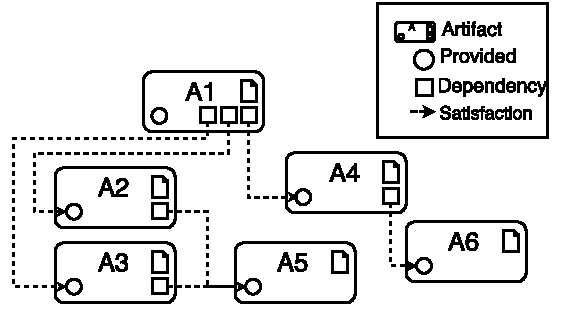
\includegraphics[width=.6\linewidth]{dependency_graph}
  \caption{Dependency Graph}
  \label{fig:dependency_graph}
\end{figure}

\begin{algorithm}
 \KwIn{A goal}
 \KwResult{DeploymentPlan plan}
 \caption{doPlanDeployment(Goal goal)}
 \label{alg:deployment_plan}

 List [] artifacts $\leftarrow$ getArtifactsThatProvide(goal)\;
 \ForEach{Artifact artifact in artifacts}{
   	Boolean contextSatisfaction $\leftarrow$ isSatisfied(artifact.contextConditions)\;
    \If{contextSatisfaction}{
      DeploymentPlan plan $\leftarrow$ new DeploymentPlan()\;
      \ForEach{Goal dependency in artifact.dependencies}{
          DeploymentPlan subPlan  $\leftarrow$ doPlanDeployment(dependency)\;
          \If{!dependencySatisfaction == NULL}{
            \Return{NULL}
          }\Else{
            plan.add(subPlan);
          }
      }
      \Return{plan}
    }\Else{
      \Return{NULL}
    }
  }
\end{algorithm}



% \chapter{Evaluation}
% \chapter{Conclusion}

\postextual
\anexos


\bibliographystyle{plain}
\bibliography{bibliografia}
\end{document}
